\documentclass[14pt]{extbook}
\usepackage{multicol, enumerate, enumitem, hyperref, color, soul, setspace, parskip, fancyhdr} %General Packages
\usepackage{amssymb, amsthm, amsmath, bbm, latexsym, units, mathtools} %Math Packages
\everymath{\displaystyle} %All math in Display Style
% Packages with additional options
\usepackage[headsep=0.5cm,headheight=12pt, left=1 in,right= 1 in,top= 1 in,bottom= 1 in]{geometry}
\usepackage[usenames,dvipsnames]{xcolor}
\usepackage{dashrule}  % Package to use the command below to create lines between items
\newcommand{\litem}[1]{\item#1\hspace*{-1cm}\rule{\textwidth}{0.4pt}}
\pagestyle{fancy}
\lhead{Progress Quiz 3}
\chead{}
\rhead{Version A}
\lfoot{3148-2249}
\cfoot{}
\rfoot{Spring 2021}
\begin{document}

\begin{enumerate}
\litem{
Write the equation of the graph presented below in the form $f(x)=ax^2+bx+c$, assuming  $a=1$ or $a=-1$. Then, choose the intervals that $a, b,$ and $c$ belong to.
\begin{center}
    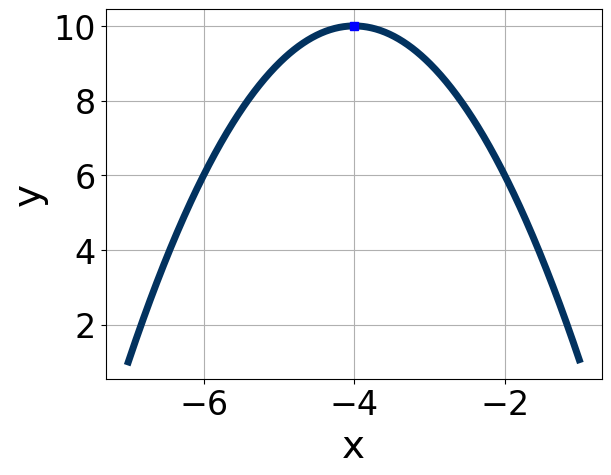
\includegraphics[width=0.5\textwidth]{../Figures/quadraticGraphToEquationCopyA.png}
\end{center}
\begin{enumerate}[label=\Alph*.]
\item \( a \in [-1.4, 0.1], \hspace*{5mm} b \in [-9, -7], \text{ and } \hspace*{5mm} c \in [-28, -22] \)
\item \( a \in [0.7, 1.8], \hspace*{5mm} b \in [7, 11], \text{ and } \hspace*{5mm} c \in [8, 10] \)
\item \( a \in [0.7, 1.8], \hspace*{5mm} b \in [-9, -7], \text{ and } \hspace*{5mm} c \in [8, 10] \)
\item \( a \in [-1.4, 0.1], \hspace*{5mm} b \in [7, 11], \text{ and } \hspace*{5mm} c \in [-28, -22] \)
\item \( a \in [-1.4, 0.1], \hspace*{5mm} b \in [7, 11], \text{ and } \hspace*{5mm} c \in [-8, -4] \)

\end{enumerate} }
\litem{
Factor the quadratic below. Then, choose the intervals that contain the constants in the form $(ax+b)(cx+d); b \leq d.$\[ 16x^{2} -32 x + 15 \]\begin{enumerate}[label=\Alph*.]
\item \( a \in [2.4, 6.4], \hspace*{5mm} b \in [-8, -2], \hspace*{5mm} c \in [3.33, 5.5], \text{ and } \hspace*{5mm} d \in [-3, 4] \)
\item \( a \in [6.4, 11.5], \hspace*{5mm} b \in [-8, -2], \hspace*{5mm} c \in [1.84, 2.76], \text{ and } \hspace*{5mm} d \in [-3, 4] \)
\item \( a \in [-1.2, 1.5], \hspace*{5mm} b \in [-23, -19], \hspace*{5mm} c \in [0.68, 1.66], \text{ and } \hspace*{5mm} d \in [-14, -10] \)
\item \( a \in [1.5, 2.8], \hspace*{5mm} b \in [-8, -2], \hspace*{5mm} c \in [6.85, 8.23], \text{ and } \hspace*{5mm} d \in [-3, 4] \)
\item \( \text{None of the above.} \)

\end{enumerate} }
\litem{
Factor the quadratic below. Then, choose the intervals that contain the constants in the form $(ax+b)(cx+d); b \leq d.$\[ 36x^{2} +60 x + 25 \]\begin{enumerate}[label=\Alph*.]
\item \( a \in [16.95, 18.02], \hspace*{5mm} b \in [4, 6], \hspace*{5mm} c \in [1.7, 2.5], \text{ and } \hspace*{5mm} d \in [3, 6] \)
\item \( a \in [5.95, 6.23], \hspace*{5mm} b \in [4, 6], \hspace*{5mm} c \in [5.59, 6.05], \text{ and } \hspace*{5mm} d \in [3, 6] \)
\item \( a \in [1.06, 2.49], \hspace*{5mm} b \in [4, 6], \hspace*{5mm} c \in [16.72, 18.55], \text{ and } \hspace*{5mm} d \in [3, 6] \)
\item \( a \in [-0.31, 1.65], \hspace*{5mm} b \in [30, 38], \hspace*{5mm} c \in [-1.03, 1.65], \text{ and } \hspace*{5mm} d \in [26, 32] \)
\item \( \text{None of the above.} \)

\end{enumerate} }
\litem{
Write the equation of the graph presented below in the form $f(x)=ax^2+bx+c$, assuming  $a=1$ or $a=-1$. Then, choose the intervals that $a, b,$ and $c$ belong to.
\begin{center}
    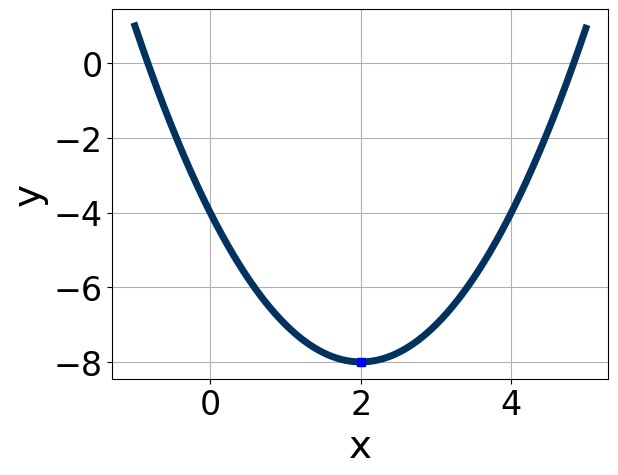
\includegraphics[width=0.5\textwidth]{../Figures/quadraticGraphToEquationA.png}
\end{center}
\begin{enumerate}[label=\Alph*.]
\item \( a \in [-2, 0], \hspace*{5mm} b \in [-8, -6], \text{ and } \hspace*{5mm} c \in [-8, -6] \)
\item \( a \in [1, 2], \hspace*{5mm} b \in [7, 11], \text{ and } \hspace*{5mm} c \in [23, 25] \)
\item \( a \in [-2, 0], \hspace*{5mm} b \in [7, 11], \text{ and } \hspace*{5mm} c \in [-8, -6] \)
\item \( a \in [1, 2], \hspace*{5mm} b \in [-8, -6], \text{ and } \hspace*{5mm} c \in [23, 25] \)
\item \( a \in [1, 2], \hspace*{5mm} b \in [-8, -6], \text{ and } \hspace*{5mm} c \in [8, 10] \)

\end{enumerate} }
\litem{
Solve the quadratic equation below. Then, choose the intervals that the solutions $x_1$ and $x_2$ belong to, with $x_1 \leq x_2$.\[ 25x^{2} -50 x + 24 = 0 \]\begin{enumerate}[label=\Alph*.]
\item \( x_1 \in [19.9, 20.15] \text{ and } x_2 \in [29.5, 30.02] \)
\item \( x_1 \in [0.27, 0.51] \text{ and } x_2 \in [2.05, 2.58] \)
\item \( x_1 \in [0.49, 0.62] \text{ and } x_2 \in [1.24, 1.98] \)
\item \( x_1 \in [0.2, 0.39] \text{ and } x_2 \in [3.75, 4.61] \)
\item \( x_1 \in [0.69, 0.82] \text{ and } x_2 \in [0.82, 1.36] \)

\end{enumerate} }
\litem{
Solve the quadratic equation below. Then, choose the intervals that the solutions belong to, with $x_1 \leq x_2$ (if they exist).\[ -18x^{2} -12 x + 2 = 0 \]\begin{enumerate}[label=\Alph*.]
\item \( x_1 \in [-0.7, 1.2] \text{ and } x_2 \in [0.22, 0.98] \)
\item \( x_1 \in [-1.5, -0.5] \text{ and } x_2 \in [-0.85, 0.42] \)
\item \( x_1 \in [-17.5, -16.4] \text{ and } x_2 \in [16.16, 16.82] \)
\item \( x_1 \in [-3.4, -1] \text{ and } x_2 \in [14.4, 14.58] \)
\item \( \text{There are no Real solutions.} \)

\end{enumerate} }
\litem{
Solve the quadratic equation below. Then, choose the intervals that the solutions belong to, with $x_1 \leq x_2$ (if they exist).\[ -11x^{2} +14 x -2 = 0 \]\begin{enumerate}[label=\Alph*.]
\item \( x_1 \in [-11.76, -8.76] \text{ and } x_2 \in [10.6, 13.6] \)
\item \( x_1 \in [0.16, 4.16] \text{ and } x_2 \in [0.5, 1.6] \)
\item \( x_1 \in [-2.11, -0.11] \text{ and } x_2 \in [-0.8, 0.9] \)
\item \( x_1 \in [-13.2, -10.2] \text{ and } x_2 \in [-2.4, -0.9] \)
\item \( \text{There are no Real solutions.} \)

\end{enumerate} }
\litem{
Graph the equation below.\[ f(x) = (x+3)^2 + 12 \]\begin{enumerate}[label=\Alph*.]
\begin{multicols}{2}\item 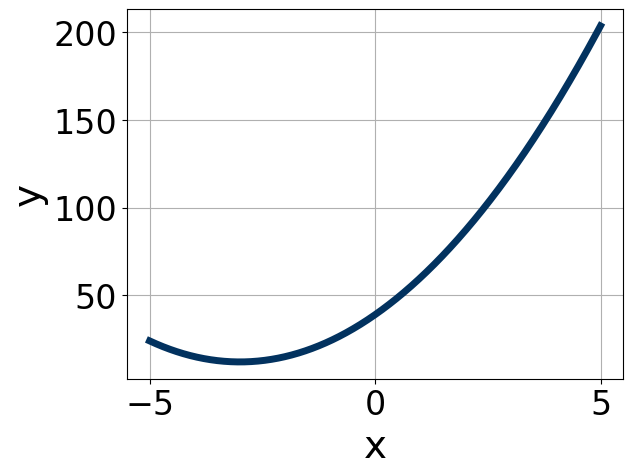
\includegraphics[width = 0.3\textwidth]{../Figures/quadraticEquationToGraphCopyAA.png}\item 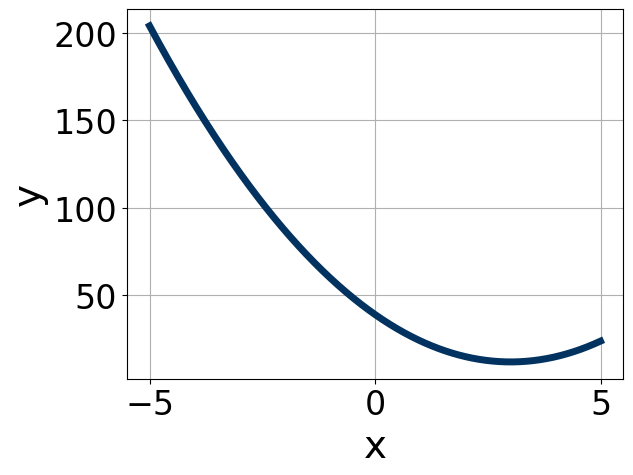
\includegraphics[width = 0.3\textwidth]{../Figures/quadraticEquationToGraphCopyBA.png}\item 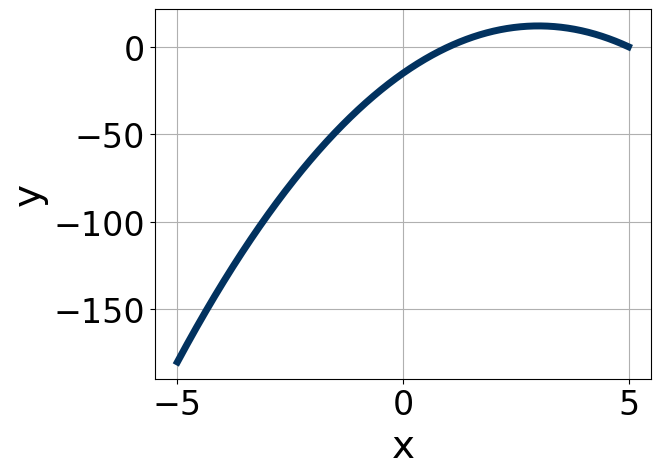
\includegraphics[width = 0.3\textwidth]{../Figures/quadraticEquationToGraphCopyCA.png}\item 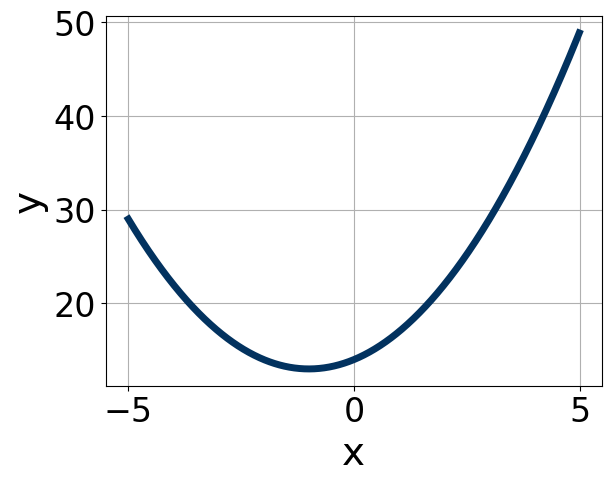
\includegraphics[width = 0.3\textwidth]{../Figures/quadraticEquationToGraphCopyDA.png}\end{multicols}\item None of the above.
\end{enumerate} }
\litem{
Graph the equation below.\[ f(x) = (x-1)^2 - 10 \]\begin{enumerate}[label=\Alph*.]
\begin{multicols}{2}\item 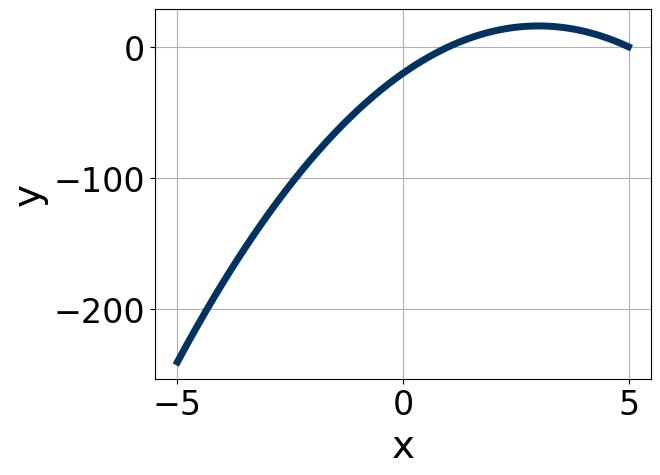
\includegraphics[width = 0.3\textwidth]{../Figures/quadraticEquationToGraphAA.png}\item 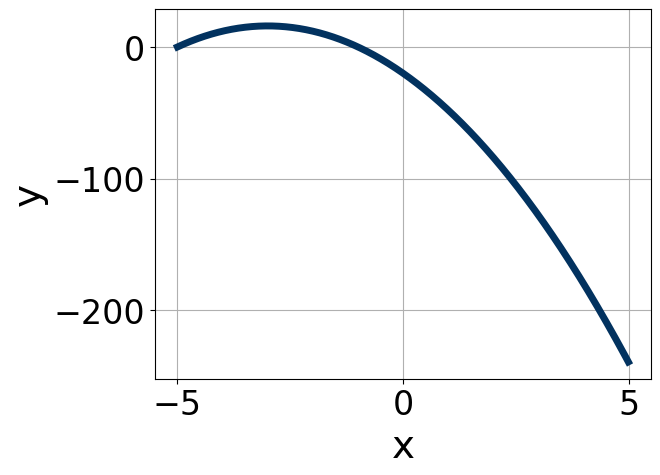
\includegraphics[width = 0.3\textwidth]{../Figures/quadraticEquationToGraphBA.png}\item 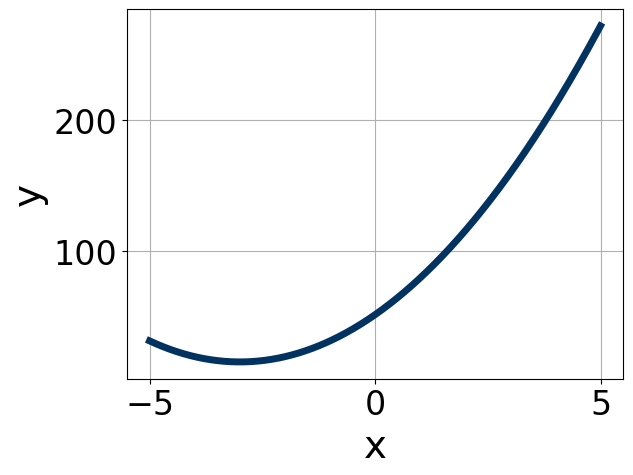
\includegraphics[width = 0.3\textwidth]{../Figures/quadraticEquationToGraphCA.png}\item 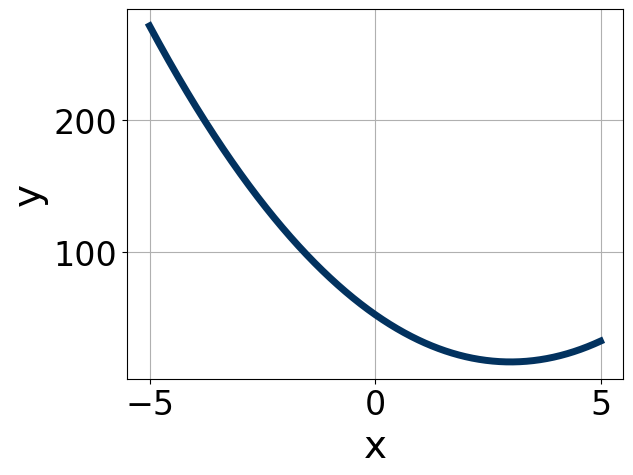
\includegraphics[width = 0.3\textwidth]{../Figures/quadraticEquationToGraphDA.png}\end{multicols}\item None of the above.
\end{enumerate} }
\litem{
Solve the quadratic equation below. Then, choose the intervals that the solutions $x_1$ and $x_2$ belong to, with $x_1 \leq x_2$.\[ 25x^{2} -60 x + 36 = 0 \]\begin{enumerate}[label=\Alph*.]
\item \( x_1 \in [1.18, 1.37] \text{ and } x_2 \in [-0.03, 1.83] \)
\item \( x_1 \in [0.1, 0.32] \text{ and } x_2 \in [5.96, 6.91] \)
\item \( x_1 \in [0.57, 0.64] \text{ and } x_2 \in [1.46, 3.25] \)
\item \( x_1 \in [29.81, 30.09] \text{ and } x_2 \in [28.84, 31.15] \)
\item \( x_1 \in [0.29, 0.42] \text{ and } x_2 \in [3.49, 4.12] \)

\end{enumerate} }
\end{enumerate}

\end{document}